\chapter{5 Things Elon Musk Could Change About Twitter}

These notes follow a School of Hard Knocks interview, curated by LazyingArt LLC, and read the talk as a sequence of entrepreneurial design conjectures rather than as settled platform history. The speaker does not write equations on a board, so when we introduce formal notation we are only making explicit the bookkeeping and incentive logic already implicit in the transcript: first motive, then bots, authentication, speech rules, creator pay, algorithmic openness, and finally the edit button as a problem of record integrity.

\section{Why the Acquisition Matters}

We begin where the lecture begins: the purchase of Twitter is described as a split decision in public opinion. Some users are excited, some are worried, and that disagreement is not treated as the endpoint of the discussion. Instead, it is used to open a more interesting question. If a highly visible operator buys a platform that he already uses heavily, and if some of his posts have moved markets, then the acquisition is unlikely to be casual. It must be attached to purpose, responsibility, and a view of how the platform ought to work.

That is the first important move in the lecture. We are not being asked merely whether we like the purchase. We are being asked to infer what sort of redesign an owner might attempt. The speaker briefly widens the frame by pointing to Musk's other companies and to the claim that they are meant to improve the world in some way. Then he narrows the discussion again and promises a five-part breakdown. This is the real start of the chapter. From here on, the lecture becomes a study of platform design.

\section{Bots, Metric Inflation, and Going Private}

\paragraph{Anecdote.}
The first change is introduced from everyday experience. We are asked to imagine a familiar scene under a popular post: suspicious accounts, thin activity histories, recently created profiles, spammy comments, scammy behavior. The lecturer starts here because the audience can recognize the symptom immediately.

\paragraph{Mechanism.}
He then pivots from symptom to structure. The claim is that bots are not merely unpleasant. They also enter the platform's counts. If they like, retweet, comment, and post, then they inflate the public-facing measures by which a platform appears to be thriving.

\begin{definition}
We let
\[
E_{\mathrm{rep}}
\]
denote reported engagement and
\[
M_{\mathrm{rep}}
\]
denote reported monthly active users. In the bookkeeping implicit in the lecture, these can be decomposed into authentic and bot-driven parts:
\begin{align}
E_{\mathrm{rep}} &= E_{\mathrm{auth}} + E_{\mathrm{bot}}, \\
M_{\mathrm{rep}} &= M_{\mathrm{auth}} + M_{\mathrm{bot}}.
\end{align}
These are not quoted formulas from the speaker. They are a compact transcription of the logic he uses.
\end{definition}

Once we write the matter this way, the speaker's business argument becomes transparent. If bot activity rises, then the reported numbers rise as well:
\begin{equation}
\text{Bot activity} \uparrow
\quad \Longrightarrow \quad
E_{\mathrm{rep}} \uparrow,\qquad
M_{\mathrm{rep}} \uparrow.
\end{equation}
The lecture then adds the next link in the chain: when a company is public, such numbers matter to shareholders. Higher headline engagement and higher headline monthly activity can make the company look healthier than it really is.

\paragraph{Worked example.}
We can make the point concrete with a small numerical example. Suppose a reporting window contains
\[
E_{\mathrm{auth}} = 120,\qquad E_{\mathrm{bot}} = 30,
\]
and the user count is
\[
M_{\mathrm{auth}} = 90,\qquad M_{\mathrm{bot}} = 10.
\]
Then the platform can report
\begin{equation}
E_{\mathrm{rep}} = 120 + 30 = 150,
\qquad
M_{\mathrm{rep}} = 90 + 10 = 100.
\end{equation}
If the bots are removed, the platform has not suffered a mysterious collapse. It has merely stopped counting artificial activity as if it were genuine participation.

The speaker's next conjecture follows directly from this. One reason to take the company private is to reduce the pressure to defend flattering but contaminated numbers. Private ownership, in this telling, creates room to clean the platform rather than to cosmetically improve the report.

\begin{figure}[h]
\centering
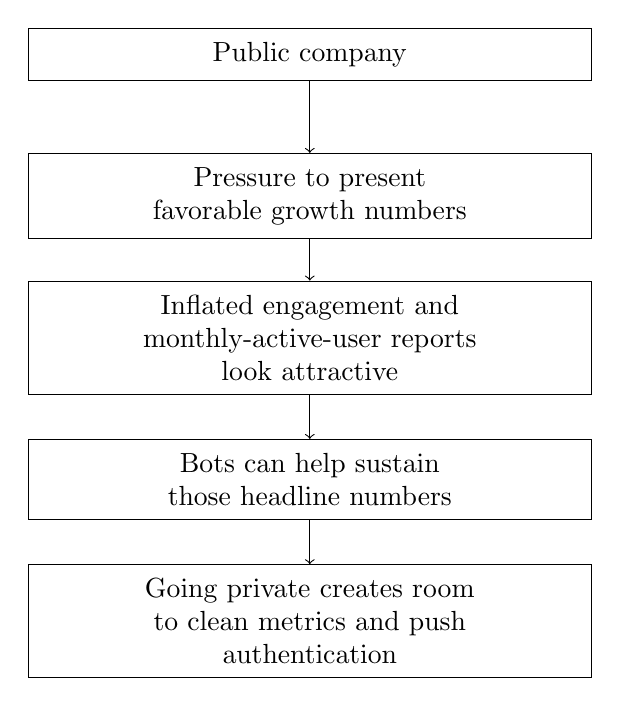
\begin{tikzpicture}
\node[draw, align=center, text width=6.8cm, inner sep=5pt] (n1) at (0,0) {Public company};
\node[draw, align=center, text width=6.8cm, inner sep=5pt] (n2) at (0,-1.8) {Pressure to present\\favorable growth numbers};
\node[draw, align=center, text width=6.8cm, inner sep=5pt] (n3) at (0,-3.6) {Inflated engagement and\\monthly-active-user reports\\look attractive};
\node[draw, align=center, text width=6.8cm, inner sep=5pt] (n4) at (0,-5.4) {Bots can help sustain\\those headline numbers};
\node[draw, align=center, text width=6.8cm, inner sep=5pt] (n5) at (0,-7.2) {Going private creates room\\to clean metrics and push\\authentication};
\draw[->] (n1) -- (n2);
\draw[->] (n2) -- (n3);
\draw[->] (n3) -- (n4);
\draw[->] (n4) -- (n5);
\end{tikzpicture}
\caption{A transcript-derived causal chain behind the lecture's argument for bot cleanup and privatization.}
\end{figure}

\paragraph{Payoff.}
The lecture does not stop with bot removal. It immediately reaches for a more durable layer beneath it. If we want clean metrics, we need not only subtraction but identification. That brings us to authentication.

\section{Authentication and a Rule-Bound Platform}

The lecturer treats authentication as the hidden infrastructure beneath several of the five predicted changes. It appears first as the natural answer to bots: verify who is actually on the platform. But it is not left there. The same device later supports moderation, creator payment, and trust in edited records.

We can express the idea in a minimal way. Let
\[
\mathcal U_A
\]
be the set of authenticated users, and let
\[
\mathcal R
\]
be the set of accounts removed or restricted for specified reasons. Then the lecture's moderation principle can be written schematically as
\begin{equation}
S(u) = S_0
\qquad
\forall\, u \in \mathcal U_A \setminus \mathcal R,
\end{equation}
where \(S(u)\) denotes the service level delivered to a user \(u\). The point is not the symbol. The point is the rule: the platform is not supposed to cater to every opinion, but it is supposed to offer the same platform service to authenticated users unless some explicit rule is triggered.

This is where the lecture turns to censorship and speech. The speaker acknowledges the anxiety around reducing censorship, but he does not frame the issue as a demand that everyone be pleased. On the contrary, he invokes a balancing image: the extreme poles on the left and right should both be unhappy. If we formalize the rhetoric only very lightly, we obtain the heuristic relation
\begin{equation}
D_L \approx D_R,
\end{equation}
where \(D_L\) and \(D_R\) are dissatisfaction levels at the political extremes. We should not overread this equation. It is not a measured law. It is a compact way of recording the lecture's intended symmetry: no side should feel uniquely protected or uniquely silenced.

The deeper move is this: once the platform can identify who is speaking, it can attempt to govern by rules rather than by opaque favoritism. That is why the speech discussion comes after the bot discussion. Identity is presented as the precondition for a more legible moderation regime.

\section{Creator Pay and the Economics of Attention}

The next shift in the lecture is from governance to incentives. If the platform is to become healthier, it should not merely remove bad activity. It should also reward productive activity. Here the speaker turns to monetization and argues that Twitter, in its present form, does not pay creators in the same way that rival platforms do.

The analogy comes from gaming. In esports and adjacent digital economies, one hears the phrase \emph{play to earn}. The lecture asks whether a related model could be brought to Twitter as a kind of \emph{tweet to earn}. The proposed mechanism is not specified in technical detail, but the logic can still be summarized:
\begin{equation}
p_i = f(a_i, g_i),
\qquad
a_i \in \{0,1\}.
\end{equation}
Here \(p_i\) is the platform-side payout to creator \(i\), \(a_i\) is an authentication flag, and \(g_i\) is the engagement attributed to that creator. The function \(f\) is deliberately unspecified because the lecture does not tell us whether engagement should mean views, likes, retweets, comments, or some weighted mixture of them.

What the speaker \emph{does} tell us is more basic. Outside Twitter, short-form platforms already compensate creators through attention-linked systems. Inside Twitter, by contrast, many accounts still rely on their own affiliate or marketing strategies rather than on a strong built-in payment rail. The proposed change is therefore entrepreneurial before it is technical. It is an attempt to turn attention into a more native platform economy.

A simple example shows why authentication returns here. Suppose two accounts generate the same measured engagement:
\[
g_1 = g_2.
\]
If account \(1\) is authenticated and account \(2\) is not, so that
\[
a_1 = 1,\qquad a_2 = 0,
\]
then the platform can at least imagine a payout system that routes revenue to creator \(1\) while withholding or delaying payout for creator \(2\) until identity is verified. Again, the lecture does not prove that Twitter \emph{will} do this. It argues that if creator payment is to become more native, authentication is the mechanism that keeps bots from collecting the checks.

The section ends with a comparison rather than a conclusion. TikTok, Reels, Shorts, and related platforms are treated as the current power players in creator monetization. Twitter, in the lecturer's forecast, could compete only by linking its text-first culture to some new payment logic, perhaps even one flavored by web3 language. The prediction is speculative, but the incentive structure is clear enough.

\section{Open-Source Algorithm and Operational Transparency}

The fourth predicted change is briefer and more declarative. The lecturer now moves from user identity and creator payment to the platform's recommendation machinery itself. If Twitter becomes more open about the way its algorithm works, creators and users gain transparency. In the lecture's framing, this is valuable in its own right.

The speaker then attaches several operational claims to this openness. Once the company is private, he suggests, it becomes easier to change the algorithm in a way that reduces maintenance cost, increases speed, makes the system more flexible, and improves security. We should record these as claims of mechanism rather than as demonstrated results. The lecture does not derive them. It presents them as the expected benefits of a more transparent and reworkable technical core.

Even here, the sequence matters. This point comes after creator pay because the talk is still asking what sort of infrastructure a redesigned platform would need. If a platform wants cleaner metrics, authenticated users, more consistent rules, and better creator incentives, then it must eventually expose or revise the machinery that determines visibility in the first place.

\section{Edit Button and Historical Integrity}

The fifth and final predicted change is the most sharply formed design problem in the lecture. An edit button looks attractive. Many users want one. The speaker notes that public polling suggests broad support for it. But he also insists that the issue is not as simple as it first appears. The real concern is not convenience. It is integrity. If a tweet can be altered after the fact, what happens to the record of what was originally said?

\subsection{Question \& Answer}

\paragraph{Question.}
How can a platform permit edits without destroying the authenticity of the original tweet?

\paragraph{Answer.}
The lecture's answer is to separate two things that are often confused: the \emph{current display} of a tweet and the \emph{history} of that tweet. The displayed version may change, but the earlier versions must remain inspectable. The speaker describes this with blockchain language, but the essential mathematical idea is simpler than blockchain. It is an append-only record.

Let a tweet \(T\) have versions
\[
T^{(0)}, T^{(1)}, \dots, T^{(n)},
\]
with \(T^{(0)}\) the original statement and \(T^{(n)}\) the current visible form. Then the version history is
\begin{equation}
H(T) = \bigl(T^{(0)}, T^{(1)}, \dots, T^{(n)}\bigr),
\qquad
T_{\mathrm{curr}} = T^{(n)}.
\end{equation}
An edit is not modeled by overwriting the past. It is modeled by appending a new state:
\begin{equation}
H_{n+1}(T) = \bigl(H_n(T),\, T^{(n+1)}\bigr),
\qquad
T_{\mathrm{curr}} \leftarrow T^{(n+1)}.
\end{equation}
The integrity condition is then immediate:
\begin{equation}
T^{(0)} \in H(T)
\quad \text{even when} \quad
T_{\mathrm{curr}} \neq T^{(0)}.
\end{equation}

This is the right place to notice how the lecture closes a circle. The platform began as a question of trust: are the users real, are the metrics real, are the moderation rules legible, are the payouts going to the right people? The edit button returns us to the same theme in textual form. Can the platform preserve authenticity while still allowing useful change?

\begin{figure}[h]
\centering
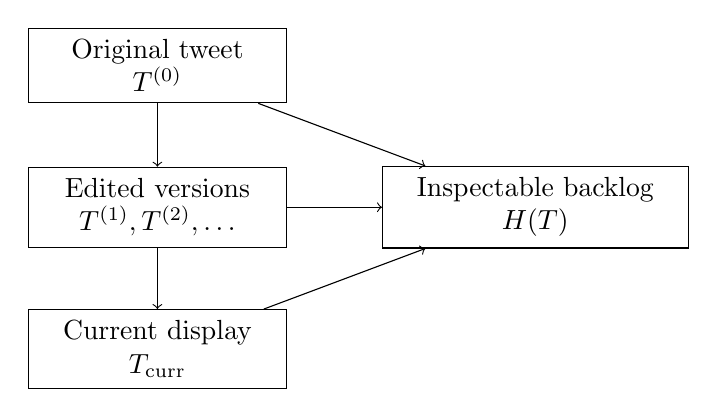
\begin{tikzpicture}
\node[draw, align=center, text width=3.0cm, inner sep=4pt] (o) at (0,0) {Original tweet\\\(T^{(0)}\)};
\node[draw, align=center, text width=3.0cm, inner sep=4pt] (e) at (0,-1.8) {Edited versions\\\(T^{(1)},T^{(2)},\dots\)};
\node[draw, align=center, text width=3.0cm, inner sep=4pt] (c) at (0,-3.6) {Current display\\\(T_{\mathrm{curr}}\)};
\node[draw, align=center, text width=3.6cm, inner sep=4pt] (h) at (4.8,-1.8) {Inspectable backlog\\\(H(T)\)};
\draw[->] (o) -- (e);
\draw[->] (e) -- (c);
\draw[->] (o) -- (h);
\draw[->] (e) -- (h);
\draw[->] (c) -- (h);
\end{tikzpicture}
\caption{A transcript-derived model of editable tweets with preserved history.}
\end{figure}

The lecture's proposal is therefore modest and precise. We need not insist on blockchain in a strict technical sense. What matters is the append-only structure. The current tweet may evolve, but its ancestry cannot disappear. In the speaker's view, that is what keeps convenience from erasing accountability.

\section{Summary}

The talk begins with public controversy and ends with record integrity, but along the way it traces a surprisingly coherent entrepreneurial architecture. First, bots corrupt the surface numbers by which the platform appears to thrive, and that creates pressure for cleaner metrics. Second, authentication becomes the hidden infrastructure that supports bot removal, rule-bound moderation, creator payment, and trust in edited records. Third, platform governance is framed not as making everyone happy, but as offering consistent service under explicit rules. Fourth, creator monetization is imagined as a more native attention economy, perhaps a kind of tweet-to-earn system, though the lecture keeps the mechanism speculative. Fifth, algorithmic openness is offered as a route to transparency and operational flexibility. Finally, the edit button becomes the lecture's sharpest design question: how do we allow revision without losing the original statement?

Read as entrepreneurship notes, the lecture is less about celebrity than about ownership as system redesign. The speaker's five predictions are really five attempts to rework incentives: what gets counted, who gets trusted, who gets heard, who gets paid, how visibility is governed, and how history is preserved.